\documentclass[11pt]{article}

\usepackage[left=0.75in, right=0.75in, top=0.75in, bottom=0.75in]{geometry}
\usepackage{layout}
\usepackage{ucs}
\usepackage[utf8x]{inputenc}
\usepackage{titlesec}
\usepackage{graphicx}
\usepackage{amssymb}
\usepackage{amsmath}
\usepackage{dsfont}
\usepackage{float}
\usepackage{caption}
\usepackage{subcaption}
\usepackage{array}



\title{\textbf{TS217 TP}\\Communications numériques multi-porteuses\\Les système OFDM}
\author{Maxime PETERLIN - \texttt{maxime.peterlin@enseirb-matmeca.fr}\\
Gabriel VERMEULEN - \texttt{gabriel@vermeulen.email} \\\\{ENSEIRB-MATMECA, Bordeaux}}
\date{27 mars 2015}


\begin{document}

\maketitle
\tableofcontents

\newpage

\section{Introduction}

L'objectif de ce TP de communications numériques est de mettre en œuvre avec MATLAB le codage OFDM dans le cadre d'un canal Rayleigh.

	\section{Hypothèses et paramètres de simulation}
		
		\begin{itemize}
			\item La modulation numérique est de type BPSK (symboles iid)
			\item Le temps symbole Ts est égale à 0.05 $\mu s$
			\item Le nombre de sous-porteuses totales N est égale à 128
			\item Le nombre de sous-porteuses utilisées $N_u$ est égale à 128
			\item Les symboles OFDM sont modulés et démodulés en utilisant respectivement les algorithmes IFFT et FFT
			\item Une trame OFDM contient $N_t$ = 500 symboles OFDM
			\item Le canal de propagation est tel que $h_l(p) = \sum\limites_{k=0}^{L-1} h_l[k] \delta [p-k]$, où les $h_l[k]$ sont iid et $h_l[k] ~ N_C(0, \frac{1}{L})$. On supposera que la réponse impulsionnelle (RI) du canal est invariante sur la durée d'une trame OFDM et que L $<<$ N
			\item La durée du préfixe cyclique est égale à $T_CP \geq LT_s$
			\item Le bruit $n_l[p] ~ N_C(0, \sigma_{n_l}^2$
			\item Les échantillons du signal OFDM, du canal et du bruit sont supposés décorrélés et indépendants
		\end{itemize}

	\section{Formalisme mathématique}
	
	\section{Implémentation de la chaîne de communication}
	
	\subsection{Validation de l'implémentation}

	La chaîne de communication implémenté sous MATLAB est testée en vérifiant que le TEB est nul lorsqu'il n'y a pas de canal et pas bruit.\\
	La courbe du TEB en fonction du bruit nous permet également d'avoir une confirmation du bon fonctionnement de notre chaîne de communication.

		\begin{figure}[h]
			\centering
			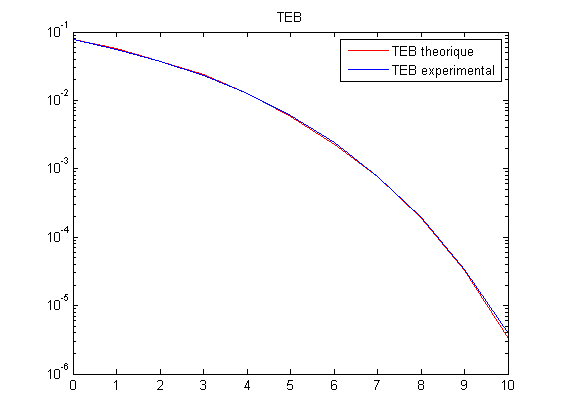
\includegraphics[scale=0.6]{img/teb.png}
			\caption{TEB en fonction du SNR}
			\label{teb}
		\end{figure}

	\subsection{Débit binaire utile}
	
		
	
	\section{Implémentation d'un égaliseur par forçage à zero}
	
	Le test de l'égaliseur se fait avec L = 16 et $\sigma_{n_l}^2$
		
		\begin{figure}[h]
			\centering
			\includegraphics[scale=0.6]{img/TEBegal.png}
			\caption{TEB en fonction du SNR}
			\label{egal}
		\end{figure}
	
	\section{Performances de la chaîne de communication}
	
		\subsection{Avec CP \geq L}
		
		\begin{figure}[h]
			\centering
			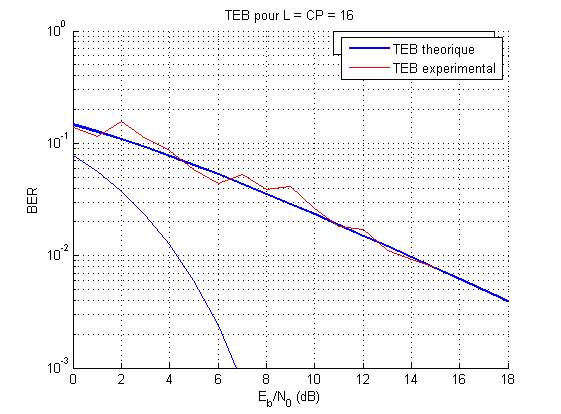
\includegraphics[scale=0.6]{img/teb1.png}
			\caption{TEB en fonction du SNR pour la nème sous-porteuse}
			\label{teb1}
		\end{figure}
		
		\subsection{Avec CP < L}

		\begin{figure}[h]
			\centering
			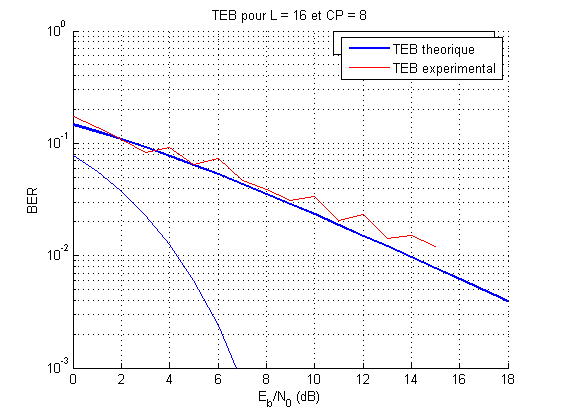
\includegraphics[scale=0.6]{img/teb2.png}
			\caption{TEB en fonction du SNR pour la nème sous-porteuse}
			\label{teb2}
		\end{figure}

\end{document}
